\chapter{Plataforma de desarrollo}
\label{cap:capitulo3}

%\begin{flushright}
%\begin{minipage}[]{10cm}
%\emph{Quizás algún fragmento de libro inspirador...}\\
%\end{minipage}\\

%Autor, \textit{Título}\\
%\end{flushright}

\vspace{1cm}

En este capítulo se definen tanto la infraestructura utilizada como los métodos, tanto a nivel software como hardware, que se han utilizado para desarrollar este trabajo.\\

\section{Plataforma hardware}
\label{sec:hw}
Para satisfacer el objetivo de crear un sistema multisensorial con las características definidas en el capítulo anterior y que además sea \textit{lowcost}, la infraestructura hardware en este trabajo se ha centrado en sistemas embebidos empotrados existentes en el mercado. Dos de los sistemas más importantes son Raspberry (Figura \ref{fig:placas}-a) y Arduino (Figura \ref{fig:placas}-b). La decisión de trabajar con Raspberry en lugar de Arduino ha estado motivada por diferentes motivos. Aunque ambas placas disponen de pines GPIO para la conexión de sensores o actuadores, Arduino no permite la conexión de cámaras, mientras que en Raspberry no solo se puede acoplar su cámara (PiCam) sino que permite conectar una webcam a través de uno de los puertos USB que tiene la placa. Arduino es un microprocesador que cuenta con su IDE, mientras que Raspberry es un microordenador completo que cuenta con su propio sistema operativo Raspbian. De esta forma el usuario final puede visualizar el resultado con la conexión de la Raspberry a una pantalla a través de su puerto HDMI.\\
\begin{figure}[h!]
  \begin{center}
    \subfigure[Raspberry Pi]{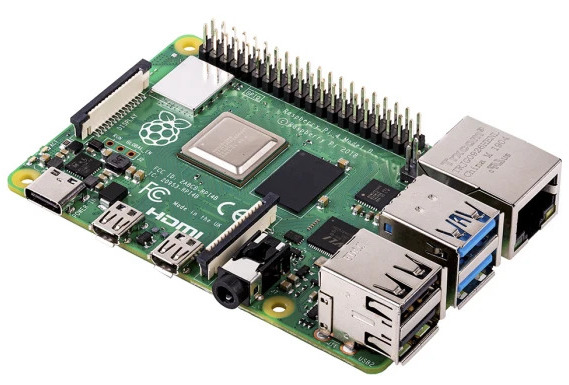
\includegraphics[width=75mm]{figs/raspberry_of}}\hspace{2mm}
    \subfigure[Arduino]{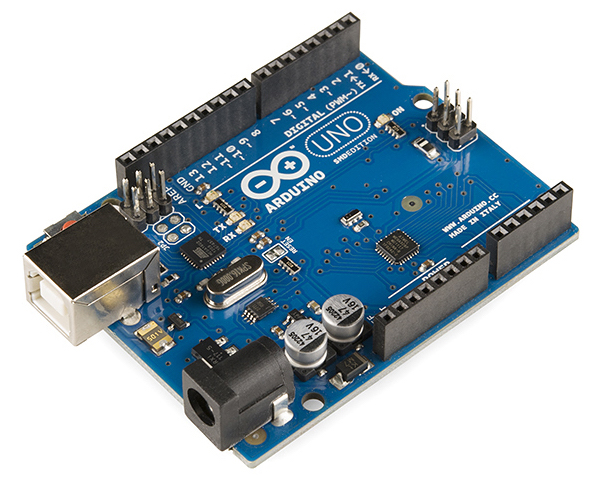
\includegraphics[width=70mm]{figs/arduino_of}}
  \end{center}
\caption{Sistemas empotrados.} \label{fig:placas}
\end{figure}

A la placa Raspberry se han conectado una serie de sensores para obtener distintos valores necesarios para la monitorización del sistema que se presentan a continuación.\\

Para la obtención de la temperatura se han utilizado el sensor BME680 (Figura \ref{fig:bme_of}) y el sensor DS18B20 (Figura \ref{fig:ds_of}). Este segundo sensor es resistente al agua, por lo que permite recoger la temperatura en superficies húmedas o mojadas. El rango en el que trabaja el BME680 así como su resolución se encuentra en el cuadro \ref{cuadro:bme_tabla} extraído de la ficha de datos del sensor. Las características del DS18B20 se encuentran en el cuadro \ref{cuadro:ds_tabla}.\\
\begin{figure} [h!]
  \begin{center}
    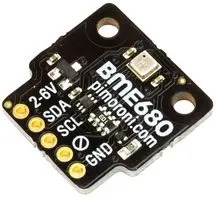
\includegraphics[width=6cm]{figs/bme_of}
  \end{center}
  \caption{Sensor BME680.}
  \label{fig:bme_of}
\end{figure}

\begin{figure} [h!]
  \begin{center}
    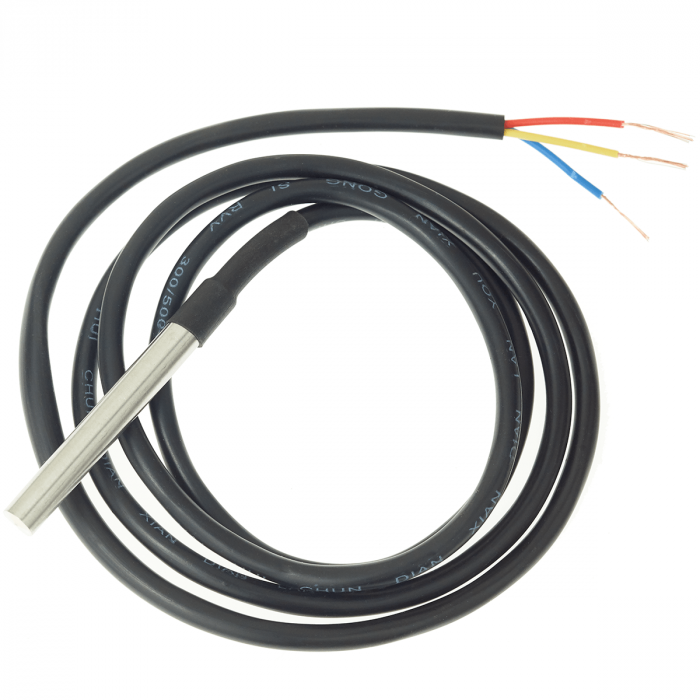
\includegraphics[width=6cm]{figs/ds_of}
  \end{center}
  \caption{Sensor DS18B20.}
  \label{fig:ds_of}
\end{figure}

\begin{table}[H]
\begin{center}
\begin{tabular}{|c|c|c|c|c|}
\hline
\textbf{Parámetros} & \textbf{Min}  & \textbf{Tipo}  & \textbf{Max}  & \textbf{Unidad}\\
\hline
Rango de temperatura de funcionamiento & -40 &  & 80 & ºC \\
Resolución de salida temperatura &  & 0.01 &  &ºC \\
Rango de presión de funcionamiento & 300 &  & 1100 & hPa \\
Resolución de salida presión &  & 0.18 &  &hPa \\
Rango de humedad de funcionamiento & 0 &  & 100 & \% r.H. \\
Resolución de salida humedad &  & 0.005 &  &\% r.H.  \\
\hline
\end{tabular}
\caption{Cuadro de características del sensor BME680.}
\label{cuadro:bme_tabla}
\end{center}
\end{table}

\begin{table}[H]
\begin{center}
\begin{tabular}{|c|c|c|c|}
\hline
\textbf{Parámetros} & \textbf{Min} & \textbf{Max}  & \textbf{Unidad}\\
\hline
Rango de temperatura de funcionamiento  & -55 & 125 & ºC \\
\hline
\end{tabular}
\caption{Cuadro de características del sensor DS18B20.}
\label{cuadro:ds_tabla}
\end{center}
\end{table}

Para la lectura de la humedad, la presión y la calidad del aire se ha utilizado el sensor BME680 (Figura \ref{fig:bme_of}), pues es capaz de medir más de un parámetro. La tabla de características se encuentra en el cuadro \ref{cuadro:bme_tabla}.\\

Para el registro de imágenes térmicas, se han utilizado dos sensores. Uno de ellos es el sensor AMG8833 (Figura \ref{fig:termicos}-a) que ofrece una matriz de valores de temperatura. El segundo es la cámara Seek Thermal (Figura \ref{fig:termicos}-b) que se ha conectado a la Raspberry a través de su puerto USB por medio de un adaptador.\\
\begin{figure}[h!]
  \begin{center}
    \subfigure[Sensor AMG8833.]{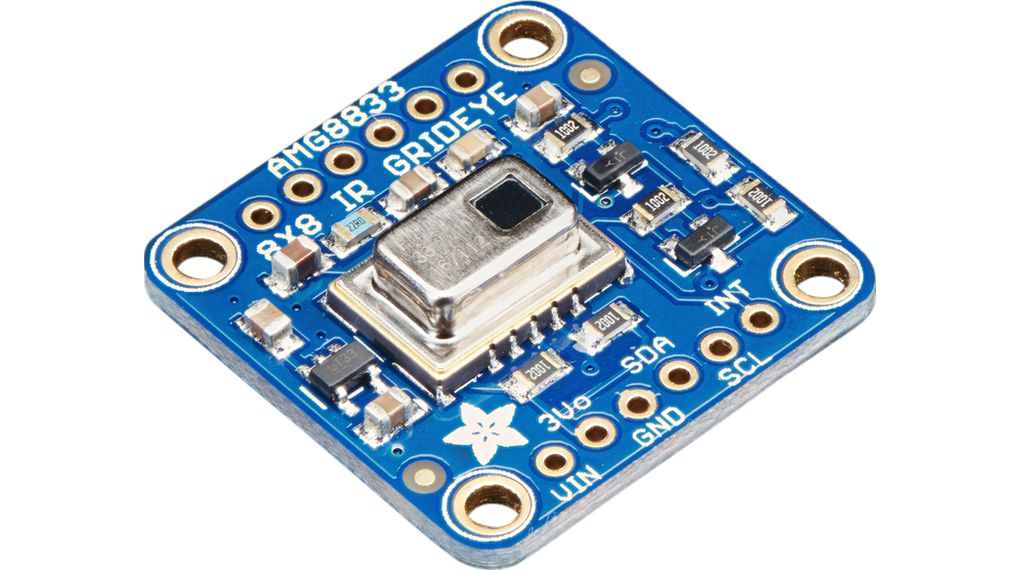
\includegraphics[width=7cm]{figs/amg_of}}\hspace{2mm}
    \subfigure[Cámara Seek Thermal]{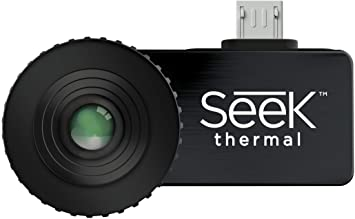
\includegraphics[width=6cm]{figs/seek_of}}
  \end{center}
\caption{Sensores térmicos utilizados en el trabajo.} \label{fig:termicos}
\end{figure}

Para el registro de imágenes se ha utilizado una de las cámaras de Raspberry, la Pi Camera (Figura \ref{fig:picam_of}). Ofrece una resolución de 8 megapíxeles, siendo una cámara de alta definición que ofrece poco ruido y alta sensibilidad.
\begin{figure} [h!]
  \begin{center}
    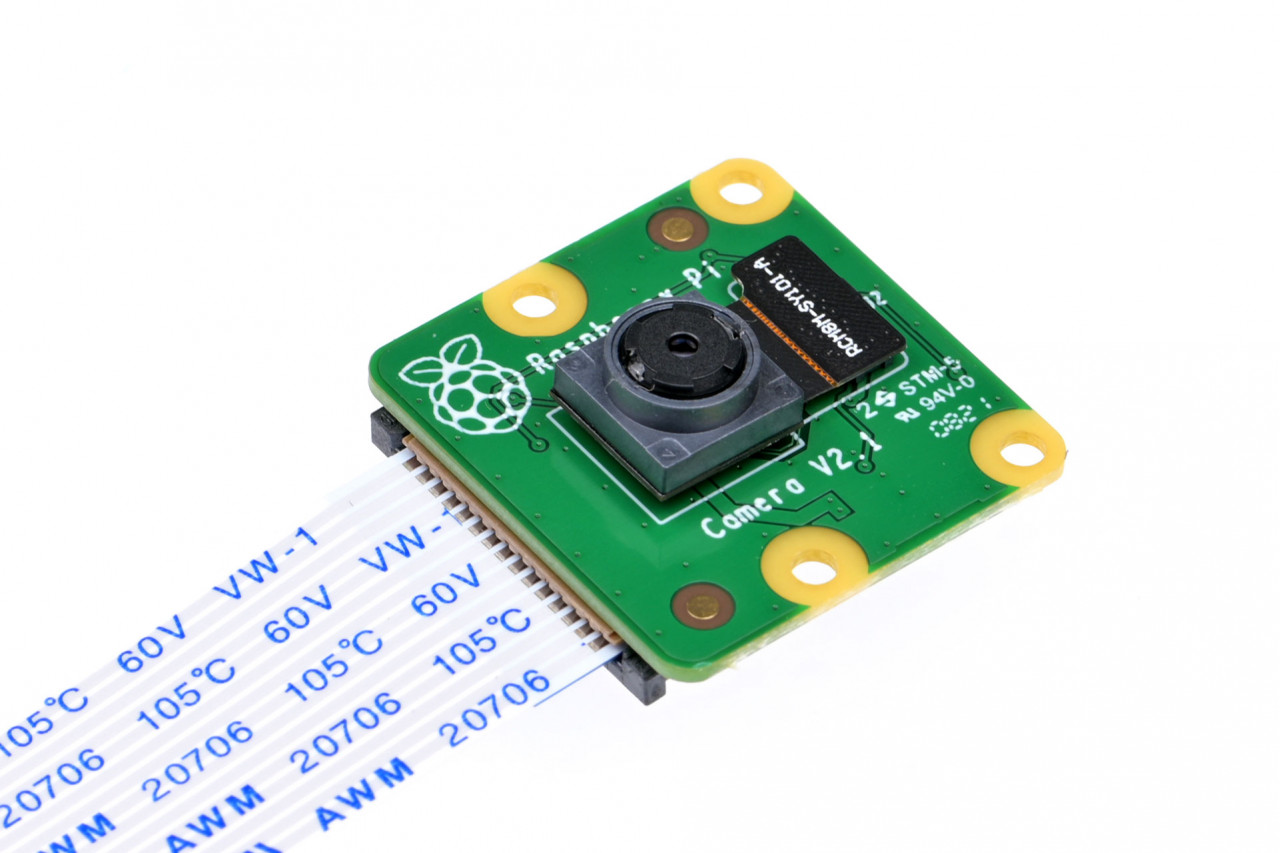
\includegraphics[width=6cm]{figs/picam_of}
  \end{center}
  \caption{Pi Camera.}
  \label{fig:picam_of}
\end{figure}

Otro sensor utilizado ha sido el sensor de nivel de agua (Figura \ref{fig:nivel_of}), que permite detectar la presencia de agua. También es posible obtener una idea de la cantidad de agua presente, aunque no de forma precisa.
\begin{figure} [h!]
  \begin{center}
    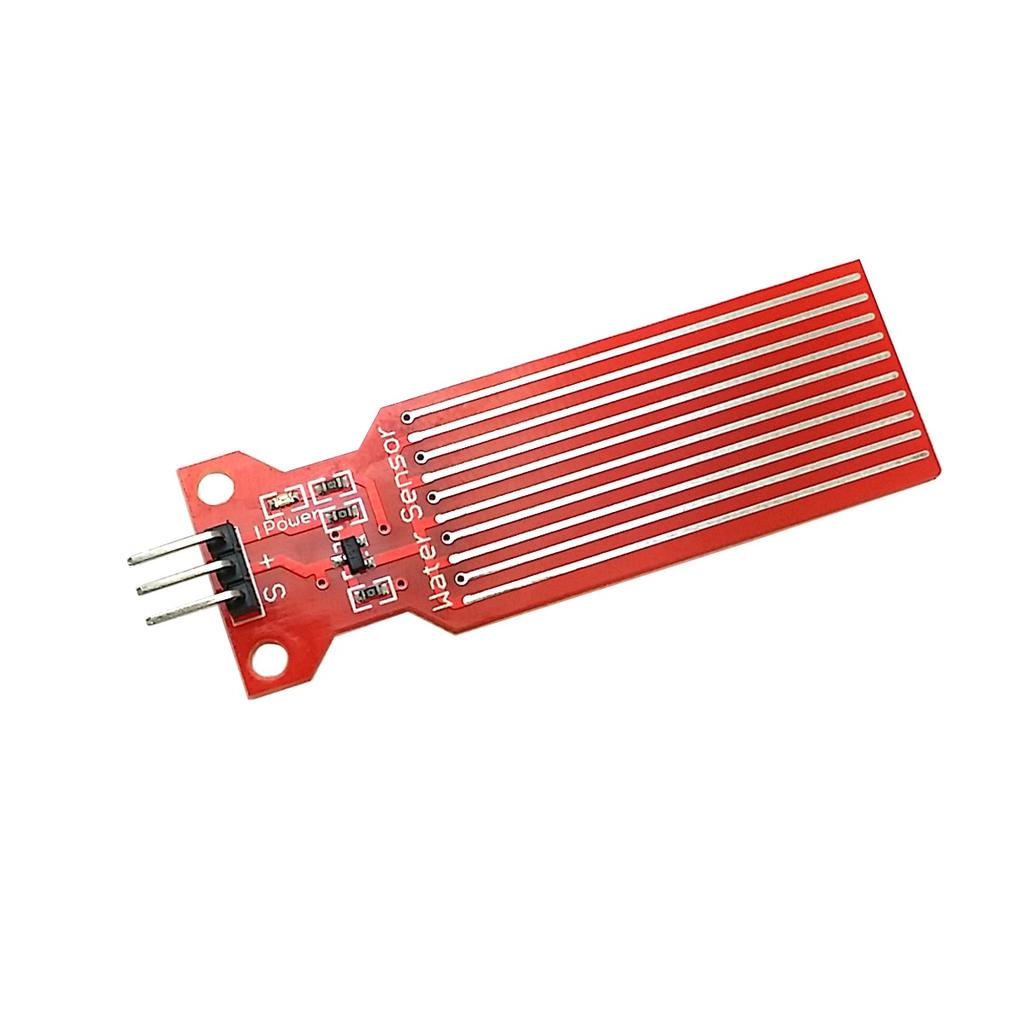
\includegraphics[width=6cm]{figs/nivel_of}
  \end{center}
  \caption{Sensor de nivel de agua.}
  \label{fig:nivel_of}
\end{figure}

El último sensor integrado en el trabajo ha sido el MQ-135 (Figura \ref{fig:mq_of}), que permite detectar la concentración de diferentes gases como el alcohol, benceno, humo, dióxido de carbono o amoníaco. En concreto, este sensor se ha utilizado para la detección de amoníaco.\\
\begin{figure} [h!]
  \begin{center}
    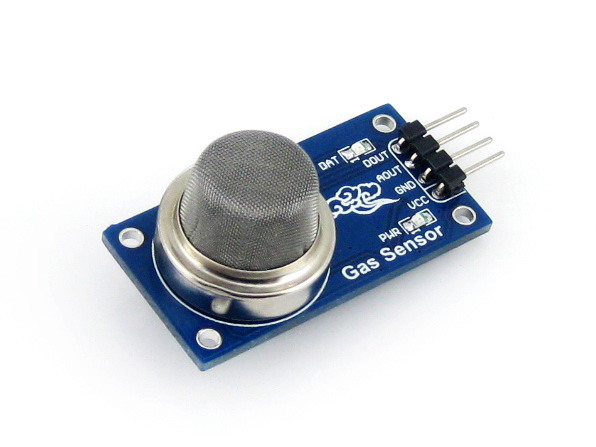
\includegraphics[width=6cm]{figs/mq_of}
  \end{center}
  \caption{Sensor MQ-135.}
  \label{fig:mq_of}
\end{figure}

Para conseguir el correcto funcionamiento de los sensores en la placa Raspberry, se ha utilizado la infraestructura software descrita a continuación.\\

\section{Infraestructura software}
Para dar soporte a la placa Raspberry se ha usado su sistema operativo oficial Raspberry Pi OS, también llamado Raspbian (Figura \ref{fig:raspbian}). La elección de usar este Sistema Operativo (SO), entre otras, es que está optimizado para funcionar en procesadores ARM, que es el que tiene Raspberry. Además, Raspberry Pi OS es el SO que mejor rendimiento ofrece para la placa.\\
\begin{figure} [h!]
  \begin{center}
    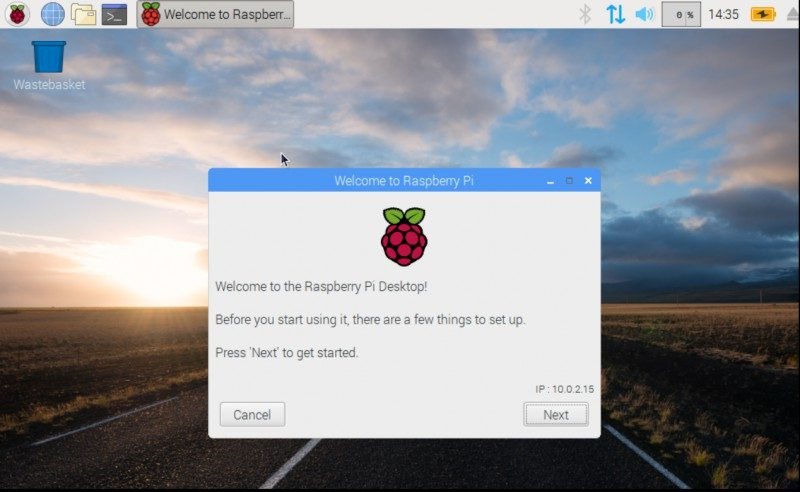
\includegraphics[width=14cm]{figs/raspbian}
  \end{center}
  \caption{Imagen de Raspberry Pi OS.}
  \label{fig:raspbian}
\end{figure}

A continuación se presentan las herramientas utilizadas para el desarrollo y funcionamiento del presente trabajo.

\subsection{Lenguaje Python}
\label{sec:python}
Python es un lenguaje de alto nivel de programación, interpretado y orientado a objetos cuya filosofía hace hincapié en la legibilidad de su código y, por ello, su sintaxis es sencilla. Ofrece numerosos módulos y librerías para las distintas aplicaciones. Algunas de estas librerías son: TensorFlow para aplicaciones en ML (Código \ref{cod:pythonML}), Pandas para análisis de datos, Flask para aplicaciones web o SQLAlchemy para comunicación entre bases de datos y programas. El uso de estos módulos y librerías facilita la reusabilidad de código y la programación modulada. No requiere del proceso de compilación, lo que lo convierte en un lenguaje muy rápido en el ciclo de edición, prueba y depuración.\\

\begin{code}[h]
\begin{lstlisting}[language=Python]
train_data = object_detector.DataLoader.from_pascal_voc('split_train_validate/train', 'split_train_validate/train', ['mouse'])
validation_data = object_detector.DataLoader.from_pascal_voc('split_train_validate/validate', 'split_train_validate/validate', 
['mouse'])
model = object_detector.create(train_data, model_spec=spec, epochs=20, batch_size=8, train_whole_model=True, validation_data=validation_data)
\end{lstlisting}
\caption[Código para generar un modelo de detección de ratones en Python]{Código para generar un modelo de detección de ratones en Python}
\label{cod:pythonML}
\end{code}

Actualmente es el lenguaje de programación más usado en el mundo según la calificación de la empresa TIOBE \footnote{\url{https://www.tiobe.com/tiobe-index/}}, por lo que cuenta con una gran comunidad. Además, también es el más popular en el ámbito del Machine Learning. Algunas de las aplicaciones que usan Python son Google, Netflix, Dropbox o Spotify.\\

La decisión de usar Python para el desarrollo de este TFG ha sido que es uno de los lenguajes de programación que mejor funciona y está soportado de forma nativa en el SO utilizado Raspbian, además de las numerosas librerías útiles para este proyecto adaptadas a Raspberry que Python posee.\\

En este trabajo, Python se utiliza para la lectura de los sensores de forma concurrente, para la creación de los dos servidores web que tiene tanto la PiCamera como la cámara térmica con Flask y para el reconocimiento de lo ratones a través de la librería TensorFlow Lite.\\

\subsection{TensorFlow Lite}
\label{sec:tensor}
TensorFlow Lite (Figura \ref{fig:tf}-a) es una variación de TensorFlow (Figura \ref{fig:tf}-b) más ligera adaptada a dispositivos como teléfonos móviles, microcontroladores o dispositivos embebidos como Raspberry. Es una plataforma de código abierto multiplataforma que permite entrenar un modelo para su posterior uso. Algunos de estos usos pueden ser la clasificación o el reconocimiento de imágenes, entre otros.\\
\begin{figure}[h!]
  \begin{center}
    \subfigure[Logo de TensorFlow Lite.]{
\includegraphics[width=7cm]{figs/tflite}}\hspace{2mm}
    \subfigure[Logo de TensorFlow]{
\includegraphics[width=6cm]{figs/tf}}
  \end{center}
\caption{} \label{fig:tf}
\end{figure}

Las características que hacen que pueda utilizarse en este tipo de dispositivos son las siguientes:
\begin{itemize}
\item{Ligereza}, ya que estos dispositivos tienen límite tanto en el almacenamiento como en la capacidad de cómputo.
\item{Baja latencia}, ya que las inferencias se realizan en el dispositivo y no en un servidor externo. 
\item{Seguridad}, debido a que el modelo viene implementado en el propio dispositivo.
\item{Consumo de energía óptimo,} dado a que no es necesario que el dispositivo esté conectado a la red, que consume mucha energía.
\end{itemize}

TensorFlow Lite se ha usado, en primer lugar, para la creación y entrenamiento de un modelo capaz de detectar ratones en una imagen (Figura \ref{fig:raton}), basándose en un dataset de 60 imágenes. En segundo lugar, para la detección de ratones en cualquier imagen o vídeo, siendo capaz de detectar el número de ratones y el lugar en el que se encuentra cada uno de ellos. Para conseguir esta detección en tiempo real del vídeo grabado por la cámara se requiere el uso de otra librería llamada OpenCV, que es descrita a continuación.\\
\begin{figure} [h!]
  \begin{center}
    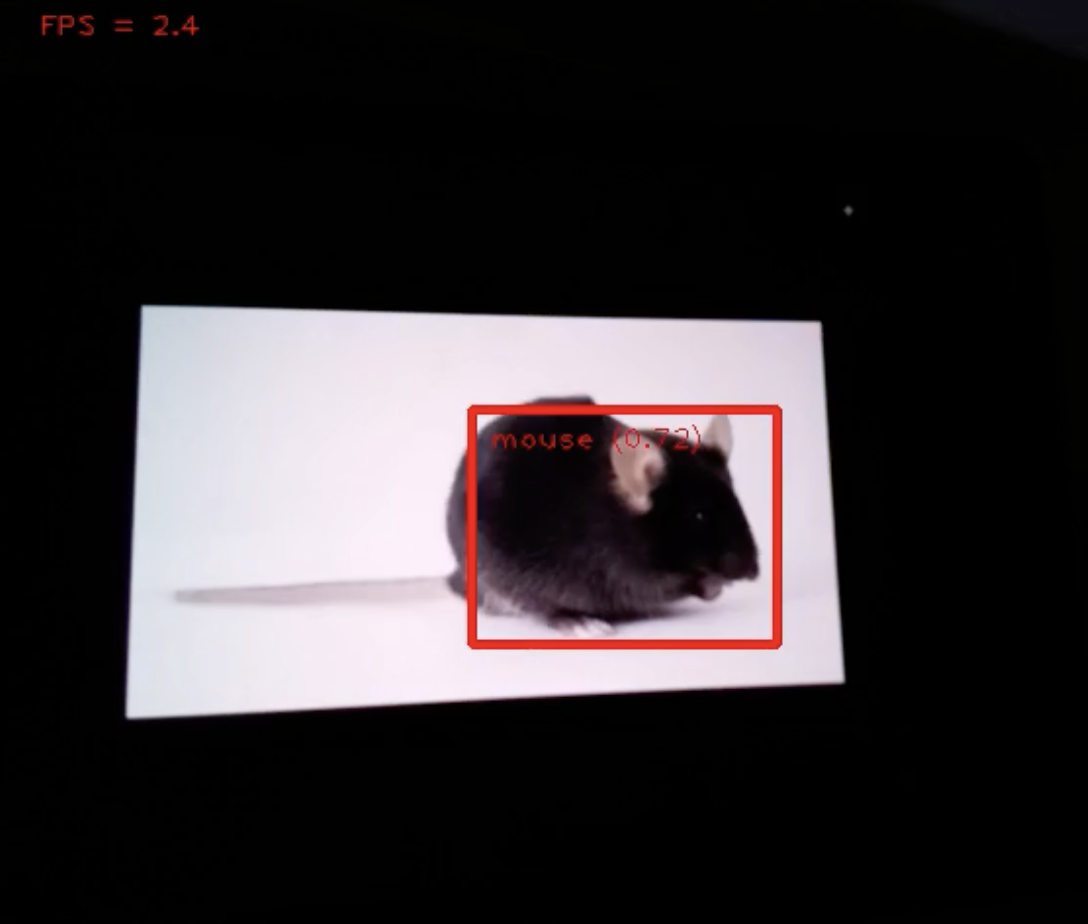
\includegraphics[width=8cm]{figs/raton-detectado}
  \end{center}
  \caption{Detección de ratones en una imagen usando TensorFlow Lite.}
  \label{fig:raton}
\end{figure}

\subsection{OpenCV}
\label{sec:opencv}
OpenCV (Open Source Computer Vision Library) es una librería de software de visión computacional y machine learning de código abierto. Es ampliamente usada en todo el mundo debido al soporte multiplataforma que ofrece para Windows, Linux, MacOS y Android, además de ofrecer interfaz en diferentes lenguajes como Python, Java, C++ y MATLAB.\\

Compuesto por más de 2500 algoritmos, OpenCV está especializado en la visión computacional y en algoritmos de aprendizaje, permitiendo reconocer rostros, identificar o clasificar objetos, extraer modelos 3D, mejorar la calidad de las imágenes o detectar bordes (Figura \ref{fig:ej-opencv}), entre otros.\\

OpenCV se ha usado en este trabajo para manipular en tiempo real los vídeos grabados por las cámaras, permitiendo ---entre otras cosas--- integrar un \textit{timestamp} en estos. También ha permitido ofrecer la funcionalidad de guardar los vídeos cuando el usuario lo solicite a través del interfaz. Por último, y dada su fácil adaptación a otras aplicaciones, ha sido posible mostrar los vídeos de ambas cámaras (térmica y RGB) en el servidor web de Flask sin problema. Esta librería se detalla a continuación.\\
\begin{figure}[h!]
  \begin{center}
    \subfigure[Imagen original]{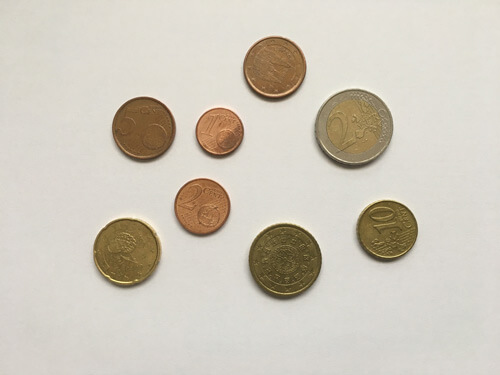
\includegraphics[width=45mm]{figs/monedas}}\hspace{9mm}
    \subfigure[Escala de grises]{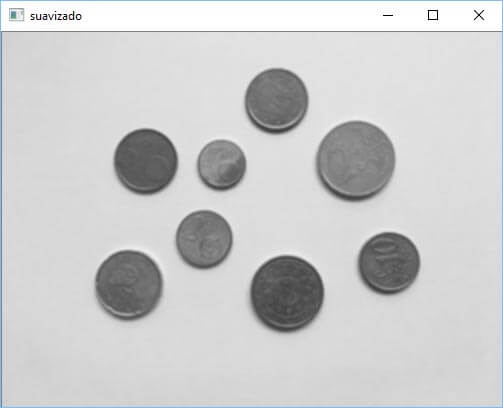
\includegraphics[width=45mm]{figs/suavizado}}\hspace{9mm}
    \subfigure[Detector de bordes]{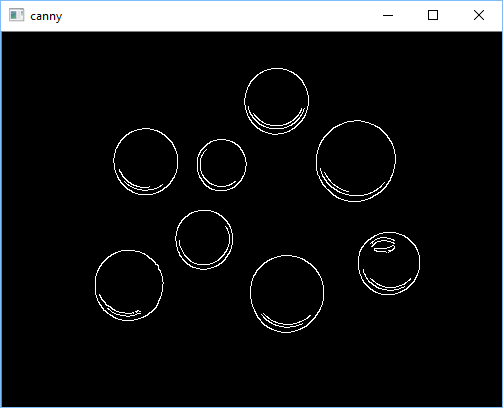
\includegraphics[width=45mm]{figs/detector-bordes}}\hspace{9mm}
    \subfigure[Contornos]{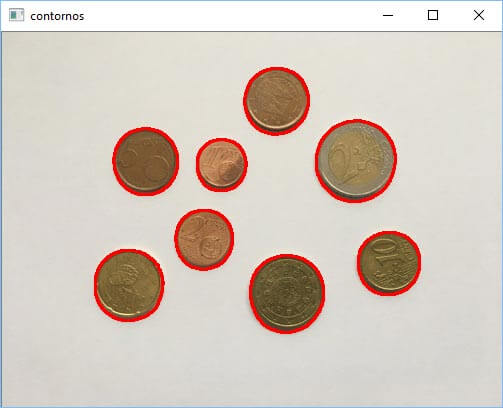
\includegraphics[width=45mm]{figs/contornos}}
  \end{center}
\caption{Ejemplo de detección de bordes con OpenCV.} \label{fig:ej-opencv}
\end{figure}

\section{Flask}
\label{sec:flask}
Flask es un marco de aplicación web minimalista ---en inglés, \textit{microframework}--- escrito en Python. Esto significa que ofrece al usuario herramientas y librerías para crear una aplicación web, y al ser minimalista, no requiere de otras dependencias para realizar las cosas básicas. Ofrece una serie de extensiones que permiten dotar de más características a la aplicación, como autenticación o manejo a través de comandos, entre otros.\\

Se compone de dos partes: las plantillas ---en inglés, \textit{templates}---, que están escritas en lenguaje HTML e indican la organización y diseño que tendrá cada página al ser visualizada, y el código en Python, que indica las rutas de cada página y las funciones de cada ruta. Este es el fichero que se ejecuta para crear el servidor.\\

En este proyecto se ha utilizado Flask para la creación de los dos servidores web de las cámaras. Se ha preferido Flask frente a Django, que es el más conocido para el uso con Python, debido a que el primero es más sencillo de utilizar y de aprender. Entre otras, este servidor permite realizar funciones como loguearse y registrase en él o acceder y controlar la visualización de las cámaras. En la Figura \ref{fig:flask-internet} se puede ver un ejemplo de un trabajo realizado con Flask.\\
\begin{figure} [h!]
  \begin{center}
    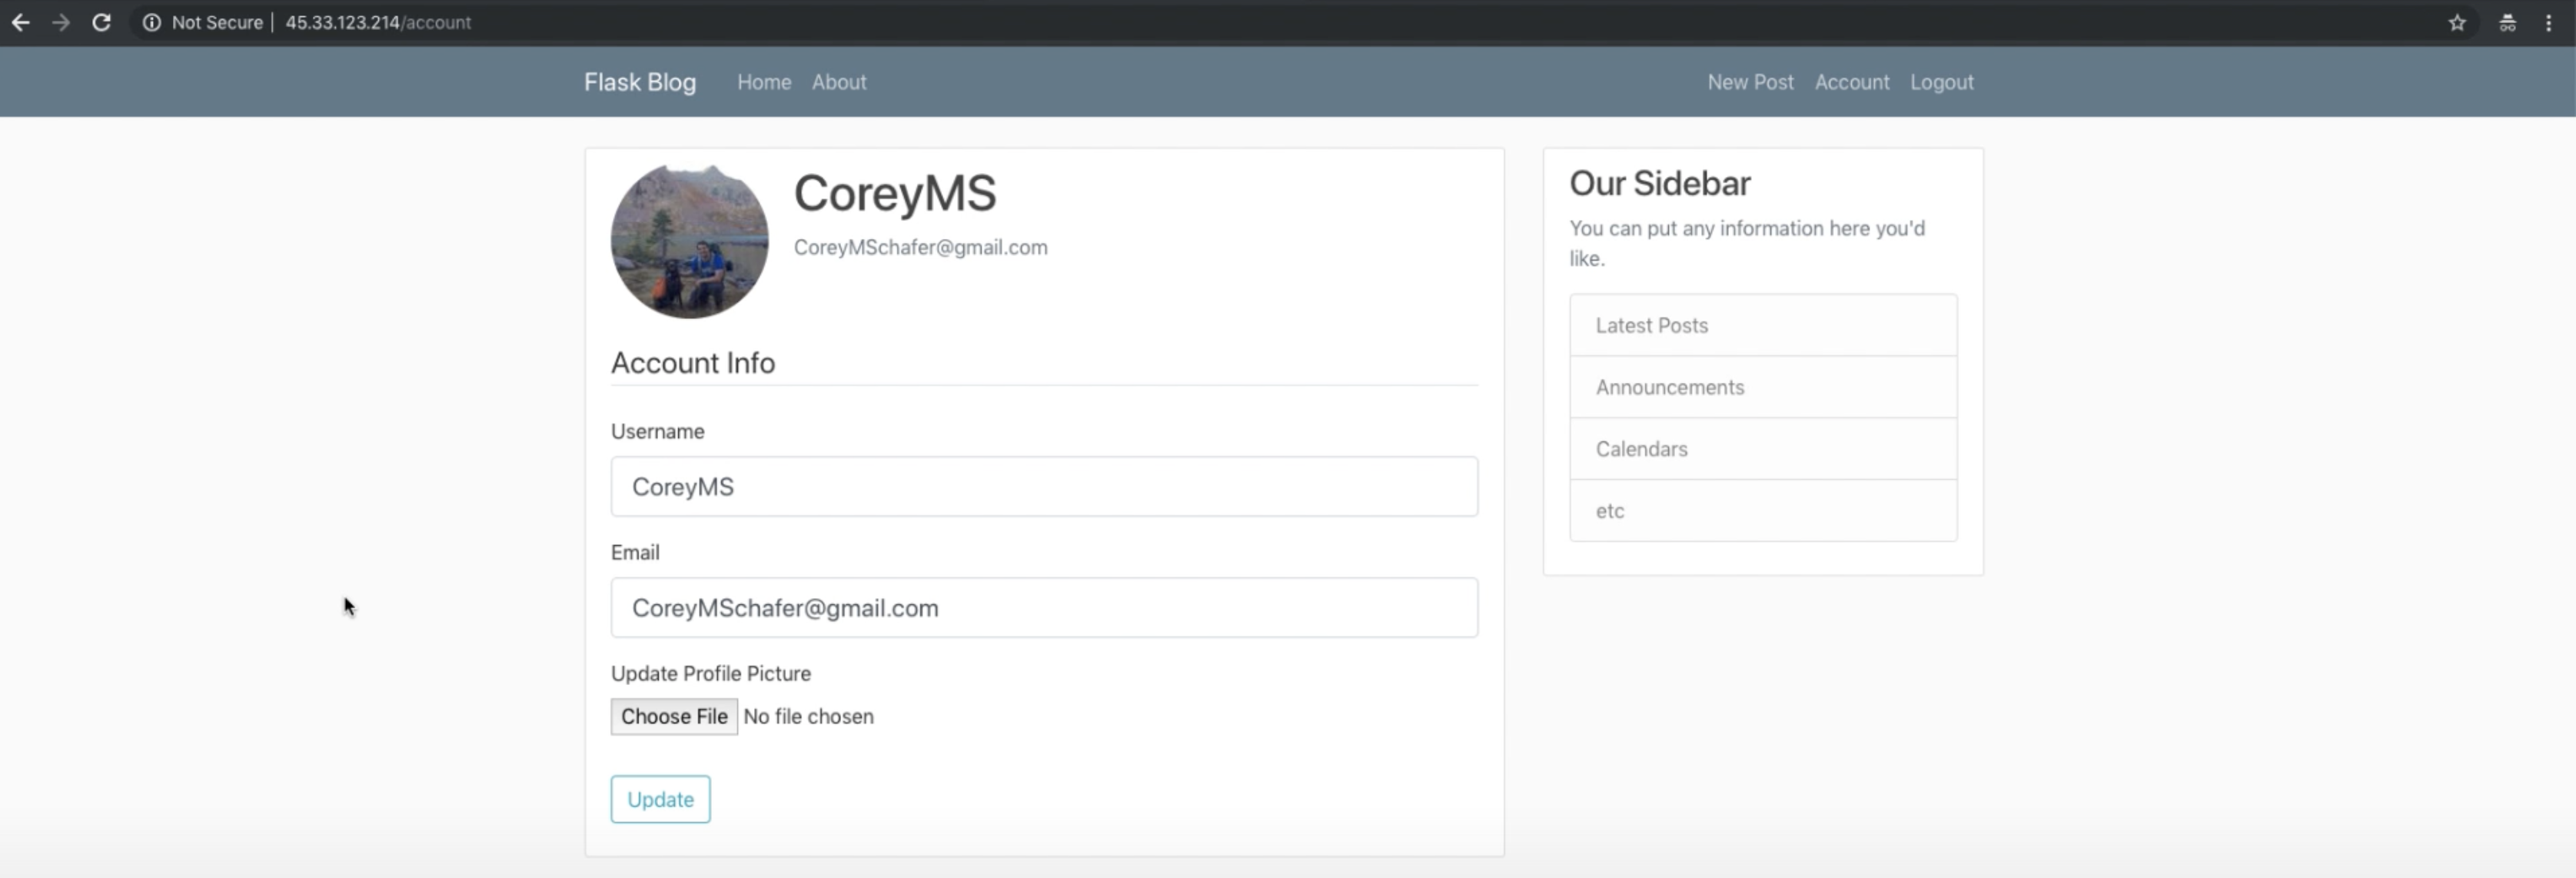
\includegraphics[width=15cm]{figs/flask-internet}
  \end{center}
  \caption{Blog creado con Flask.}
  \label{fig:flask-internet}
\end{figure}

\subsection{Node-Red}
\label{sec:nodered}
Node-Red es una herramienta de programación creada por IBM y escrita en lenguaje JavaScript que permite conectar dispositivos hardware y servicios en línea. Muestra de manera visual las conexiones de los nodos en un panel, mostrando gráficamente el flujo de la información. Además, es un entorno de ejecución ligero, lo que lo hace ideal para ejecutarse en hardware de bajo coste como la Raspberry.\\

Está compuesto por dos partes principales. Una de ellas es la edición de flujo desde navegador, donde muestra los nodos disponibles en el margen izquierdo así como la disposición y conexión del flujo creado por el usuario. La otra parte es el cuadro de mando, más comunmente \textit{dashboard}, que muestra la interfaz de usuario en base al flujo de los nodos de la parte previamente comentada.\\

Node-Red tiene una amplia variedad de nodos. Algunos de ellos permiten distintos tipos de conexiones, la interacción directa con los pines de Raspberry, la conexión con twitter o el correo electrónico. También permite la creación de ficheros de distintos tipos o la ejecución de ficheros ya existentes en la computadora.\\

Node-Red también permite el modo \textit{scripting}; esto es, la ejecución directa de código escrito en lenguaje JavaScript. Pueden crearse nuevos nodos para agregar nuevas capacidades gracias a los más de 225.000 módulos que hay en el repositorio de paquetes.\\

Los flujos de datos se pueden importar o exportar con ficheros en formato estándar JSON, permitiendo compartirlos con cualquier persona. La página de Node-Red tiene una librería de flujos que han creado otros usuarios, permitiendo el acceso a ellos para utilizarlos como base en otros proyectos (Figura \ref{fig:flujos}). En la figura \ref{fig:ui-internet} se puede ver un ejemplo de un trabajo realizado en Node-Red.\\
\begin{figure}[h!]
  \begin{center}
    \subfigure[Flujo de Hola Mundo en Node-Red]{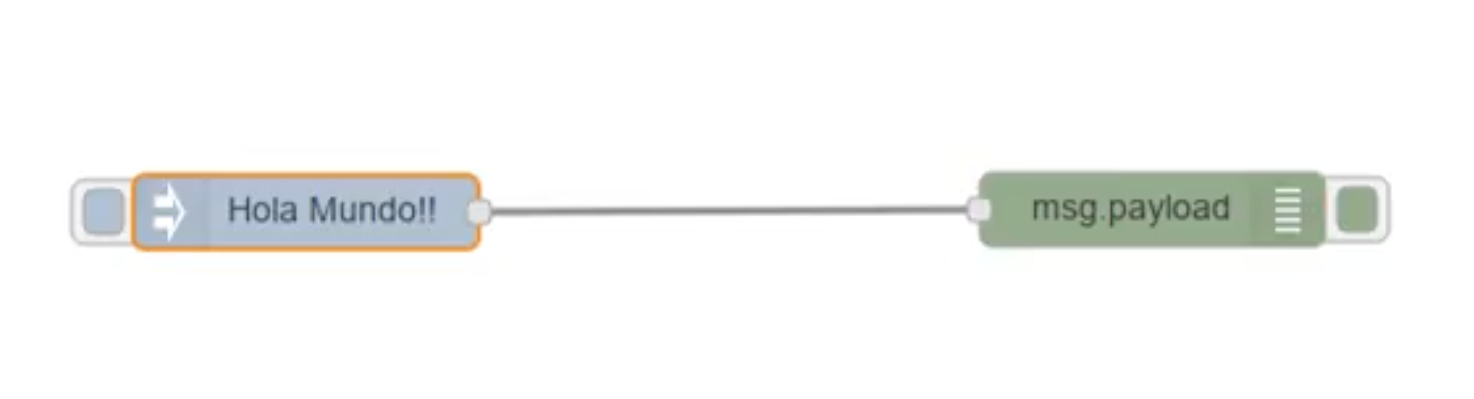
\includegraphics[width=14cm]{figs/holamundo-flujo}}\hspace{2mm}
    \subfigure[Flujo del proyecto de creación de un sistema de alarma]{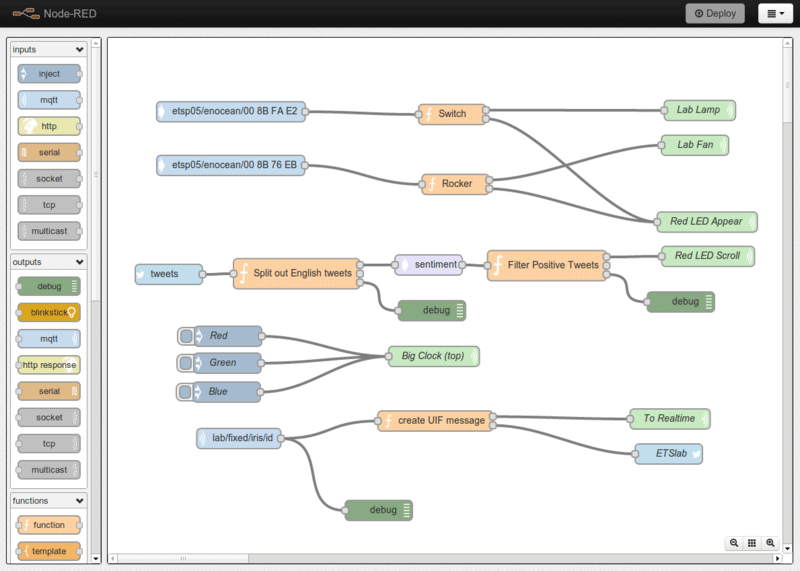
\includegraphics[width=14cm]{figs/alarma-flujo}}
  \end{center}
\caption{Distintos flujos hechos en Node-Red} \label{fig:flujos}
\end{figure}
\begin{figure} [h!]
  \begin{center}
    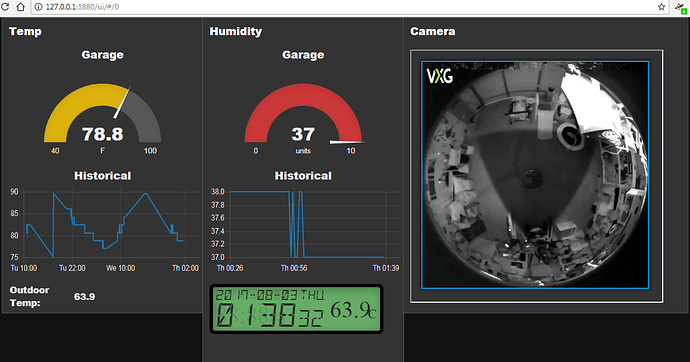
\includegraphics[width=15cm]{figs/ui-internet}
  \end{center}
  \caption{IU de un sistema de control de un garaje.}
  \label{fig:ui-internet}
\end{figure}

Para el desarrollo de este TFG, Node-Red ha tenido un papel muy importante. Además de tener una gran comunidad que permite la resolución de la mayoría de dudas, ha permitido la creación de la interfaz de usuario donde se muestran las mediciones de cada sensor, los dos servidores web de las cámaras y los botones e interruptores necesarios que permiten al usuario interactuar con la interfaz de una manera sencilla para obtener toda la información.\\